\newpage

\chapter{Chapter}

\section{Section}

\subsection{Subsection}

\subsubsection{Subsubsection}
My text here with \textit{italics}, with \textbf{bold}, and a  \href{https://davibarreira.github.io/}{link}.Adding some math expression here with $x=10$ and
\begin{displaymath}
	d(\omega(t_0),\omega(t_1)) \leq \int^{t_1}_{t_0}g(s) ds.
\end{displaymath}
Adding some code like \lstinline[style=julia]{plots}. Note that the \lstinline[style=julia]{using plots}
\begin{lstlisting}[language=JuliaLocal, style=julia]
using PlutoUI
\end{lstlisting}

\begin{lstlisting}[language=JuliaLocal, style=julia]
begin
	using Plots
  ENV["GKSwstype"] = "100"
	y(x) = sin(x)
	Plots.plot(y,
		color=:blue)
end
\end{lstlisting}

\begin{figure}[H]
	\centering
	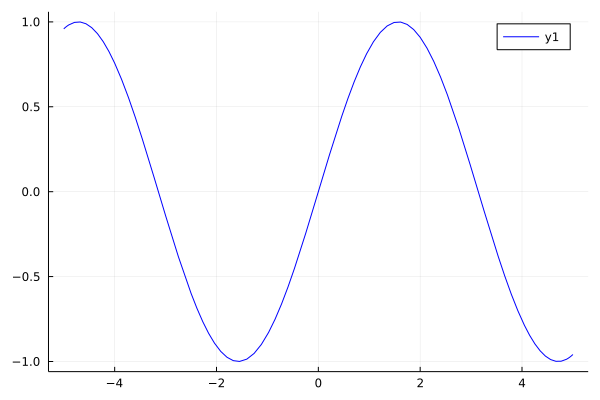
\includegraphics[width=0.8\textwidth]{./figures/notebooktest_figure1.png}
	\label{fig:notebooktest_figure1.png}

\end{figure}

\begin{lstlisting}[language=JuliaLocal, style=julia]
A = [10,10,10]
\end{lstlisting}

\begin{verbatim}
3-element Vector{Int64}:
 10
 10
 10
\end{verbatim}

\begin{lstlisting}[language=JuliaLocal, style=julia]
x = rand(10);
\end{lstlisting}

\begin{lstlisting}[language=JuliaLocal, style=julia]
x .+ 1
\end{lstlisting}

\begin{verbatim}
10-element Vector{Float64}:
 1.7163319418044432
 1.1075623003889274
 1.4148026029685155
 1.8312946938549224
 1.245318597484443
 1.3618365977661562
 1.0360493458704316
 1.691505643081338
 1.1650435473940783
 1.9755752682705847
\end{verbatim}

\begin{lstlisting}[language=JuliaLocal, style=julia]
set_theme!(theme_ggplot2())
\end{lstlisting}

\begin{lstlisting}[language=JuliaLocal, style=julia]
Makie.plot(x)
\end{lstlisting}

\begin{figure}[H]
	\centering
	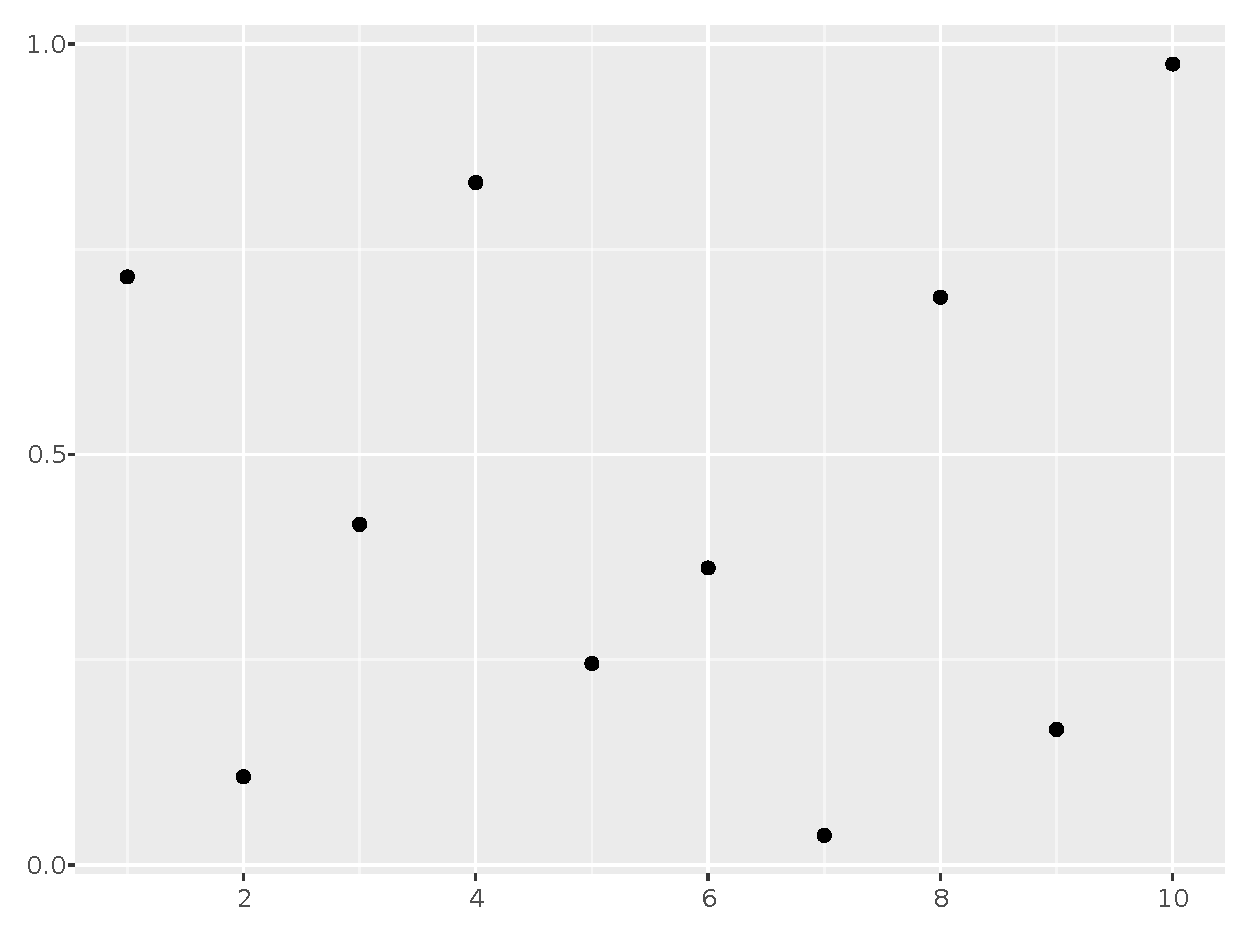
\includegraphics[width=0.8\textwidth]{./figures/notebooktest_figure2.pdf}
	\label{fig:notebooktest_figure2.pdf}

\end{figure}

\begin{lstlisting}[language=JuliaLocal, style=julia]
PlutoUI.LocalResource("./figure.svg")
\end{lstlisting}

\begin{figure}[H]
	\centering
	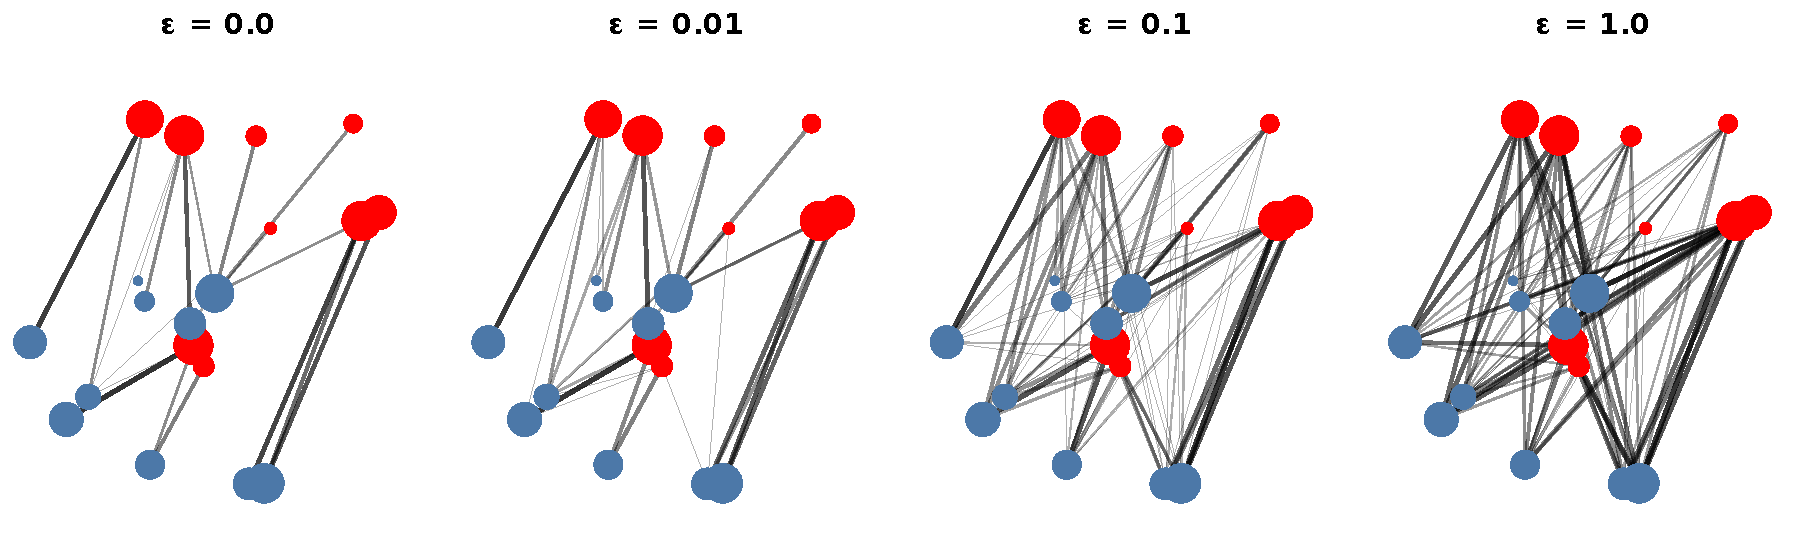
\includegraphics[width=0.8\textwidth]{./figures/figure}
	\label{fig:/home/davibarreira/MEGA/EMAp/NotebookToLatex.jl/test/pluto/./figure.svg}

\end{figure}

\begin{lstlisting}[language=JuliaLocal, style=julia]
PlutoUI.LocalResource(figurepath)
\end{lstlisting}

\begin{figure}[H]
	\centering
	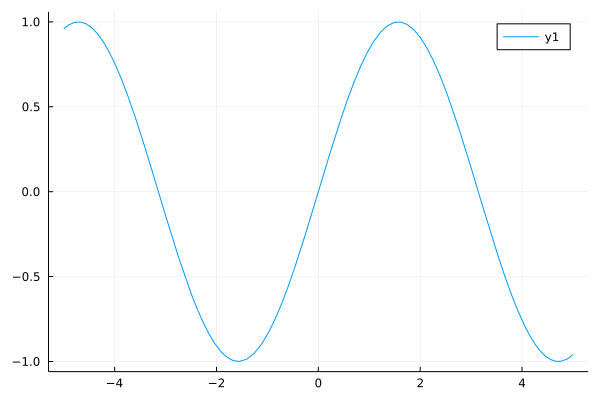
\includegraphics[width=0.8\textwidth]{./figures/plotexample.png}
	\label{fig:/home/davibarreira/MEGA/EMAp/NotebookToLatex.jl/test/pluto/plotexample.png}

\end{figure}

\begin{lstlisting}[language=JuliaLocal, style=julia]
begin
	using DataFrames
	DataFrame(a=rand(10),b=rand(["left","right"],10))
end
\end{lstlisting}

\begin{verbatim}
10×2 DataFrame
 Row │ a          b
     │ Float64    String
─────┼───────────────────
   1 │ 0.827555   left
   2 │ 0.364716   left
   3 │ 0.0366026  right
   4 │ 0.889053   right
   5 │ 0.550791   left
   6 │ 0.912717   left
   7 │ 0.43325    left
   8 │ 0.075576   left
   9 │ 0.0141365  left
  10 │ 0.453292   right
\end{verbatim}
